\documentclass[12pt]{article}

\usepackage{graphicx,booktabs}
\usepackage{subcaption,epsfig,epstopdf}
\usepackage{float}

\usepackage{pslatex,multicol,verbatim,wrapfig,pdfpages,url}

\title{Parallel Molecular Dynamics with a Time-Reversible Nos\'{e}-Hoover Thermostat on CPUs and GPUs}
%\subtitle{APC 523}

\author{Nathan Mahynski \and George A. Khoury \and Carmeline Dsilva}


\begin{document}

\maketitle

\section{Introduction}


Due to the dramatic increase in computing power over the last thirty years, molecular dynamics (MD) simulations have become a remarkably fruitful tool for scientific discovery and engineering exploration \cite{Karplus2002,Levitt2001}.
%
These simulations allow us to screen potential drug compounds \cite{Jorgensen2004}, explore protein folding dynamics \cite{Duan1998,Shaw2010,Piana2013,Lindorff-Larsen2011}, study \cite{Boero1998} and develop \cite{Zipoli2010} new catalysts, and explore extreme conditions (temperatures and pressures) that are experimentally inconvenient all without running expensive and time-consuming experiments in a laboratory.
%
Early atomistic simulations were capable of running at only short physical timescales (picoseconds \cite{Karplus1979}), but due to enhancements in algorithms, hardware, and parallelization, physically relevant timescales (milliseconds \cite{Kohlhoff2014}) can now be tractably explored on current computers.

At its core, molecular dynamics numerically integrates Newton's equation of motion ($force = mass \times acceleration$) forward in time.
%
Different numerical integration schemes result in different numerical accuracies for the simulations.
%
Standard molecular dynamics fixes the number of particles, volume, and total energy of the system.
%
However, one can introduce thermostats and barostats to the integration algorithm to adjust the temperature and pressure of the system to attempt to keep them constant (See Figure~\ref{fig:mdfigure}).

\begin{figure}
\centering
\includegraphics[width=0.65\textwidth]{mdfigure.png}
\caption{Molecular Dynamics algorithm graphical overview. MD begins with a system of particles coordinates and velocities, and integrates Newton's equation of motion forward in time utilizing a specified algorithm. A thermostat can be used to control the temperature through physics-based relationships between velocities and temperature. In this work, we implement the Nos\'{e}-Hoover Thermostat to control temperature.}
\label{fig:mdfigure}
\end{figure}

Several molecular dynamics packages exist to perform parallelized atomistic molecular dynamics simulations on CPUs.
%
These include LAMMPS \cite{Plimpton1995}, AMBER \cite{Case2010}, CHARMM \cite{MacKerell1998}, GROMACS \cite{Scott1999}, and TINKER \cite{Ponder2003}.
%
Only very recently, some of these packages have been updated in order to be implemented on Graphics Processing Units (GPUs) \cite{Brown2012,Brown2011,Gotz2012,Salomon-Ferrer2013}, and new packages exclusive to GPUs such as HOOMD-Blue\cite{Anderson2008} have been developed. %
The newly updated codes have not been nearly as extensively tested as their native CPU codebases, but can potentially offer significant speedups \url{http://ambermd.org/gpus/}.

Therefore, in this APC523 Final Project we built a new software package from scratch to run molecular dynamics simulations in parallel on both CPUs and GPUs. The GPU implementation is an ambitious goal very much working on the cutting-edge of computational science since few and only recent implementations exist on GPUs \cite{Anderson2008,Brown2012,Brown2011,Gotz2012,Salomon-Ferrer2013}.
%
The GPU implementation offers the promise of a significant speedup over CPU-only implementations.
%
The software implements the Lennard-Jones potential for interatomic interactions, a velocity-Verlet integrator, and a Nos\'{e}-Hoover thermostat. The developed software is sufficiently modular that other integration algorithms and pair potentials can easily be incorporated in future versions.
%
We chose to include the Lennard-Jones potential because many of the standard force fields \cite{Case2010,MacKerell1998,Scott1999,Kaminski2001,Arnautova2006,Khoury2013} today are built on Lennard-Jones interactions.
%
For example, a commonly used model for water, the TIP3P water model \cite{Jorgensen1983}, is composed of Lennard-Jones interactions and an additional electrostatic term to account for water's ability to be polarized.
%
In addition, Lennard-Jones particles serve as a very good model for monotomic gases such as argon \cite{Rahman1964} and condensed amorphous phases such as glasses \cite{Debenedetti2001}.

Because parallelization is essential for modern day molecular dynamics software, we implemented our software to run in parallel on both CPUs (with shared memory) and GPUs.
%
Our code is therefore fairly flexible and applicable to many different hardware architectures.

\section{Theory and Algorithms}

In the following section, we describe the theory and algorithms that underly the software developed.
%
In what follows, we assume that our system of interest consists of $N$ particles.
%
We denote the position, velocity, and acceleration of particle $i$ as $\mathbf{r}_i$, $\mathbf{v}_i$, and $\mathbf{a}_i$, respectively.
%
We denote the force on particle $i$ as $\mathbf{F}_i$.

In general, the algorithm for a molecular dynamics simulation is as follows (See Figure~\ref{fig:mdfigure}):

\begin{enumerate}
\item Initialize particle positions $\mathbf{r}_i$ and velocities $\mathbf{v}_i$ within the simulation box.
\item  \label{itm:MD_start} Calculate the forces $\mathbf{F}_i$ on each particle.
\item \label{itm:MD_end} Integrate forward the positions and velocities of each particle for the chosen timestep $\Delta t$.
\item Repeat steps \ref{itm:MD_start}-\ref{itm:MD_end} for the chosen amount of simulation time.
\end{enumerate}


% Here we show overall figure.
\subsection{Integrator} \label{subsec:integrator}

We implemented a velocity-Verlet integration algorithm \cite{Swope1982}, which is accurate to fourth order.
%
For a fixed number of particles (N), volume of the system (V), and energy (E), we update the positions and velocities of each atom using the following equations
\begin{eqnarray}
\mathbf{r}_i (t + \Delta t)  & = & \mathbf{r}_i(t) + \mathbf{v}_i(t) \Delta t + \mathbf{a}_i(t) \frac{\Delta t^2}{2} \\
\mathbf{v}_i(t + \Delta t) & = & \mathbf{v}_i(t) + \left[\mathbf{a}_i(t) + \mathbf{a}_i(t + \Delta t) \right] \frac{\Delta t}{2}
\end{eqnarray}
where $\mathbf{a}_i = \mathbf{F}_i/m$.
%
The forces can be calculated from the potential energy function and will be discussed further in subsection \ref{subsec:potential}.

Because $\mathbf{v}_i$ depends on both $\mathbf{a}_i(t)$ and $\mathbf{a}_i(t+\Delta t)$, the order of computations goes as follows
\begin{enumerate}
\item Calculate $\mathbf{r}_i(t + \Delta t)$ from $\mathbf{r}_i(t)$, $\mathbf{v}_i(t)$, and $\mathbf{a}_i(t)$.
\item Calculate $\mathbf{a}_i(t + \Delta t)$ from $\mathbf{r}_i(t + \Delta t)$.
\item Calculate $\mathbf{v}_i(t + \Delta t)$ from $\mathbf{v}_i(t)$, $\mathbf{a}_i(t)$, and $\mathbf{a}_i(t + \Delta t)$.
\end{enumerate}

\subsection{Thermostats} \label{subsec:thermostat}
The equations in \ref{subsec:integrator} are only for NVE simulations.
%
If we are instead interested in fixing temperature (T) rather than energy (E), we must introduce the idea of a {\em thermostat} to our simulations.
%
A thermostat is necessary in most simulations since experiments are not typically done at constant energy.
%
The thermostat adjusts the velocities of the particles so that they (on average) maintain a user-specified desired temperature.

We implemented a time-reversible Nos\'{e}-Hoover thermostat in our molecular dynamics software.
%
The Nos\'{e}-Hoover thermostat adjusts the particle velocities based on the target temperature of the system and the current kinetic energy of the system.
%
The thermostat is governed by its own equation of motion given by the position ($\xi$), velocity ($\dot{\xi}$), and acceleration ($\ddot{\xi}$) of the thermostat.

Let $T_{set}$ be the desired temperature.
%
Then the acceleration of the thermostat is given by
\begin{equation}
\ddot{\xi} = \frac{1}{Q} \left[ \sum_{i=1}^{N} m_i v_i^2 - N_f k_B T_{set} \right]
\end{equation}

The equations of motion for the particles and the thermostat are
\begin{eqnarray}
r_i(t + \Delta t) &=& r_i(t) + v_i(t) \Delta t + \left[ a_i(t) - v_i(t)\dot{\xi}(t) \right] \frac{\Delta t^2}{2}\\
v_i(t + \Delta t) &=& v_i(t) + \left[ a_i(t) - v_i(t) \dot{\xi}(t) \right] \frac{\Delta t}{2} + \left[a_i(t + \Delta t)  - v_i(t + \Delta t) \dot{\xi}(t + \Delta t) \right] \frac{\Delta t}{2} \\
\xi(t + \Delta t) & = & \xi(t) + \dot{\xi}(t) \Delta t + \ddot{\xi}(t) \frac{\Delta t^2 }{2} \\
\dot{\xi}(t + \Delta t)  & = & \dot{\xi}(t) + \left[ \ddot{\xi}(t) + \ddot{\xi} (t + \Delta t)  \right] \frac{\Delta t}{2}
\end{eqnarray}

The Nos\'{e}-Hoover thermostat can be shown to be time-reversible when it is implemented via the following algorithm.
First, update the thermostat velocity using a half-step in time
\begin{equation}
\dot{\xi} (t+ \Delta t/2) = \dot{\xi}(t) + \ddot{\xi}(t) \frac{\Delta t}{2}
\end{equation}
and thermostat position.
\begin{equation}
\xi (t+ \Delta t) = \xi(t) + \dot{\xi}(t+\Delta t/2)\Delta t
\end{equation}
Second, evolve the particle velocities with a half-step.
\begin{equation}
v_i (t+\Delta t/2) = v_i (t) \exp^{-\dot{\xi}(t+\Delta t/2) \Delta t/2} + a_{i} (t) \Delta t/2
\end{equation}
Third, evolve particle positions.
\begin{equation}
r_{i} (t+\Delta t) + r_{i} (t) + v_{i}(t+ \Delta t/2) \Delta t
\end{equation}
Fourth, call the function \textbf{calcForce} to update the accelerations at the next timestep.
\begin{equation}
a_{i} (t+\Delta t) = F_{i} (t+ \Delta t)/m_{i}
\end{equation}
Fifth, evolve the particle velocities.
\begin{equation}
v_{i} (t+ \Delta t)  = [v_{i}(t+\Delta t/2) + a_{i}(t+\Delta t) \Delta t/2]\exp^{-\dot{\xi}(t+\Delta t/2) \Delta t/2}
\end{equation}
Finally, the thermostat velocity is updated.
\begin{equation}
\dot{\xi}(t+\Delta t) = \dot{\xi} (t+\Delta t/2) + \ddot{\xi} (t+\Delta t) \Delta t /2
\end{equation}
The thermostat acceleration, $\ddot{\eta}(t)$ is expressed in the form
\begin{equation}
\ddot{\xi}(t) = \frac{1}{\tau^{2}} [\frac{T(t)}{T_{target}} -1 ]
\end{equation}
where $\tau^{2} = \frac{Q}{(3N-1)*T_{target}}$ and $Q$, which is the thermal mass of the thermostat spring equal to unity.
Because this algorithm is time-reversible, this algorithm is implemented in our software.
% END OF THAT DOC.

The ability for this algorithm to be time-reversible is the result of a Trotter factorization of the Liouville propagator derived by Martyna and coworkers 20 years ago. Through their Trotter factorization they proved that any resulting integrator will be time-reversible \cite{Tuckerman1992}.

\subsection{Pair potentials} \label{subsec:potential}

We implemented a shifted Lennard-Jones pair potential in our molecular dynamics software.
%
In the shifted Lennard-Jones potential, the potential energy of interaction between two particles is a function of the interatomic distance $r = \|\mathbf{r}_i - \mathbf{r}_j \|$, and is given by
\begin{equation}
U(r) = 4 \epsilon\left[ \left( \frac{\sigma}{r-\delta} \right)^{12} - \left( \frac{\sigma}{r-\delta} \right)^6 \right] + U_{shift}
\end{equation}
where $\epsilon$, $\sigma$, $\delta$, and $U_{shift}$ are adjustable parameters.
%
The total potential energy of the system is then given by
\begin{equation}
U_{tot} = \sum_{i=1}^{N} \sum_{j=1}^{i-1} U\left( \| r_i - r_j \| \right)
\end{equation}

The force on a particle $F_i$ is the gradient of the potential, $F_i = \nabla_i U_{tot}$.
%
It can be shown that
\begin{equation}
F_{i, x} = \sum_{j \ne i} \frac{d U\left( \| r_i - r_j \| \right)}{d \| r_i - r_j \| } \frac{x_i - x_j}{\|r_i - r_j\|}.
\end{equation}

The potential energy and force calculations involve $\mathcal{O}(N^2)$ calculations, since each of the $N$ particles interacts with the remaining $N-1$ particles.
%
Therefore, the potential energy and force calculation are the portions that are typically parallelized in an MD code.

\subsection{Parallelization}

We implemented parallelization on CPUs and GPUs in our molecular dynamics software.
%
On CPUs, we parallelized our code using OpenMP and therefore, our code can run in parallel on any shared memory cluster.
%
On GPUs, we parallelized our code using CUDA.
The parallelization on GPUs is implemented in the force calculation, which accounts for 27\% percent of the cost of the simulation according to our profiling studies (see Table\ref{tab:profiling}).
%
Parallelization and scaling were tested on the Adroit and TIGER clusters.

\subsection{Neighbor Lists}

\subsection{Testing}

We implemented Google Tests within our software.

We implemented the following tests:
	\begin{itemize}
	\item[\texttt{NumAtoms}] verifies that the system class stores the correct number of atoms
	\item[\texttt{KineticEnergy}] calculates the kinetic energy for a two-atom system, and verifies that it is correctly returned by the KinE() function
	\item[\texttt{PotentialEnergy}] calculates the potential energy for a two-atom system, and verifies that it is correctly returned by the PotE() function
	\item[\texttt{ChangeBox}] changes the length of the simulation box and verifies that the box is correctly changed in the system definition
	\item[\texttt{PBC}] computes the distance between two particles using the minimum image convention and verifies that it is correctly computed for different scenarios (out of box, inside box, etc.)
	\end{itemize}

Additionally, we benchmarked/validated our code's results against LAMMPS \cite{Plimpton1995}, described later in this report.

\section{Code Structure and Implementation Notes}

The software is implemented in object-oriented C++ and version-controlled through an actively updated github repository \url{https://github.com/PrincetonUniversity/CBEMDGPU}. The code is completely documented using Doxygen in the /doc directory, which contains both an html and a pdf document (\textbf{refman.pdf}) outlining the code structure and commenting all of the functions in the software.
%
The class structure is as follows
\begin{description}

\item[\texttt{common.h}] This class implements the error catching functions.

\item[\texttt{cudaHelper.h}] This function implements the CUDA code for parallelization on GPUs.

\item[\texttt{cellList.cpp}] This class controls the cell lists (for parallelization on CPU) or neighbor lists (for parallelization on GPUs).

\item[\texttt{dataTypes.h}] This function implements the custom structures, such as the atom struct, which stores the position, velocity, and acceleration of an atom.
	
\item[\texttt{integrator.cpp}] This class is a ``virtual'' class

\item[\texttt{nve.cpp}] This class implements the velocity-Verlet integration scheme for an NVE simulation.

\item[\texttt{nvt.cpp}] This class implements the velocity-Verlet integration scheme with a time-reversible Nos\'{e}-Hoover thermostat for an NVT simulation.

\item[\texttt{potential.cpp}] The potential class implements the force and potential energy calculations for the standard Lennard-Jones potential.
%
This class can be expanded to include other potential energy functions.

\item[\texttt{system.cpp}] This class stores all of the parameters relevant to the simulation system, such as the box size, potential energy function, and the number of atoms.

\item[\texttt{utils.cpp}] This class implements the necessary ``helper'' functions for the simulation, such as the distance calculation with periodic boundary conditions using the minimum image convention.

\item[\texttt{main.cpp}] This is the main driver program to run the software.

\item[\texttt{unittests.cpp}] This file implements Google Tests for our software.
%
We used a test fixture to initialize the same system construct for multiple tests.

\end{description}

\subsection{Optimizations}
This section provides an overview of the optimizations performed in our software to lead to the final submitted version.
\textbf{Nate will go through and list them by going through the different CPP files.}
\section{Results}

\subsection{Profiling}

Profiling was performed on the TIGER computer cluster using gprof with a number of different processor, skin radius, and particle combinations. We found that using 4 processors, 400 particles, a skin radius of 0.5 for 100 steps produced the most representative results. The software was compiled using the \textit{-pg} compiler option. The top 7 most expensive components of the software are presented in Table~\ref{tab:profiling}.

% Table generated by Excel2LaTeX from sheet 'Sheet1'
\begin{table}[htbp]
  \centering
  \tiny
  \caption{table son}
    \begin{tabular}{ccccccc}
    \toprule
    \% time & Cum Seconds & Self Seconds & \# of Calls & Self (s/call) & Total (s/call) & Name \\
    \midrule
    26.86 & 1.3   & 1.3   & 101   & 0.01  & 0.05  & integrator::calcForce(systemDefinition\&) \\
    17.05 & 2.13  & 0.83  & 6125941 & 0     & 0     & pbcDist2(float3 const\&, float3 const\&, float3\&, float3 const\&) \\
    15.5  & 2.88  & 0.75  & 34484119 & 0     & 0     & std::vector<float3, std::allocator<float3> >::operator[](unsigned long) \\
    10.74 & 3.4   & 0.52  & 5702835 & 0     & 0     & slj(float3 const*, float3 const*, float3*, float3 const*, float const*, float const*) \\
    8.27  & 3.8   & 0.4   & 10997635 & 0     & 0     & cellList\_cpu::list(int) const \\
    7.23  & 4.15  & 0.35  & 11617957 & 0     & 0     & std::vector<int, std::allocator<int> >::operator[](unsigned long) const \\
    4.75  & 4.38  & 0.23  & 12810108 & 0     & 0     & std::vector<atom, std::allocator<atom> >::operator[](unsigned long) \\
    \bottomrule
    \end{tabular}%
  \label{tab:profiling}%
\end{table}%

The \textbf{calcForce} function consisted of the most expensive function in the program, followed by \textbf{pbcDist2}. The function calls to the shifted lennard-jones \textbf{slj} potential and cellLists that are maintained on the CPU \textbf{cellList\_cpu}. It would be expected that the \textbf{calcForce} function utilizes the majority of the computing time and this has been observed elsewhere in MD codes. Due to the expense of this function, this function was parallelized on the GPUs.

\subsection{Scaling Studies}

We performed several scaling studies on both the TIGER and ADROIT clusters.
Tiger timing\_results.txt.tiger
\url{/home/gkhoury/APC523/project/tmp/CBEMDGPU}

for low numbers of particles scaling really  perform well because there is a lot of communication overhead.
this is expected.
for large numbers of particles we scale and this is good.

\subsection{Benchmarking and Validation against Literature Values}

\textbf{WE NEED A MSD PLOT HERE}

We validated our code against LAMMPS \cite{Plimpton1995} (http://lammps.sandia.gov), an existing and widely-used and tested commercial molecular dynamics software package.
%
We simulated a system of 4000 Lennard-Jones particles at a reduced temperature $T=0.71$.
%
We used a cubic box with edge length $L=16.796$, so that the reduced density of the system $\rho = 0.8442$.
%
We used a timestep $\Delta t=0.005$, and simulated for $10,000$ timesteps.


We compared the temperature, potential energy, total energy, and radial distribution function for the simulations calculated in our package against LAMMPS.
%
The results are shown in Figure~\ref{fig:lmp_compare} and Table~\ref{table:lmp_compare}.
%

\begin{table}
\begin{centering}
	\begin{tabular}{| r | c | c |}
		\hline
		 & CBEMDGPU & LAMMPS \\
		 \hline
		 T & 0.7104 & 0.7112 \\
		 \hline
		 Potential energy / atom & -5.6532 & -5.6594 \\
		 \hline
		 Total energy / atom & -4.5879 & -4.5929 \\
		 \hline
	\end{tabular}
	\caption{Comparison of average thermodynamic quantities for CBEMDGPU and LAMMPS simulations.}
	\label{table:lmp_compare}
\end{centering}
\end{table}

\begin{figure}[H]
	\begin{subfigure}{0.5\textwidth}
    \includegraphics[width=\textwidth]{T_compare}
	\caption{}
	\end{subfigure}
	\begin{subfigure}{0.5\textwidth}
	\includegraphics[width=\textwidth]{PE_compare}
	\caption{}
	\end{subfigure}
	\begin{subfigure}{0.5\textwidth}
	\includegraphics[width=\textwidth]{E_compare}
	\caption{}
	\end{subfigure}
	\begin{subfigure}{0.5\textwidth}
	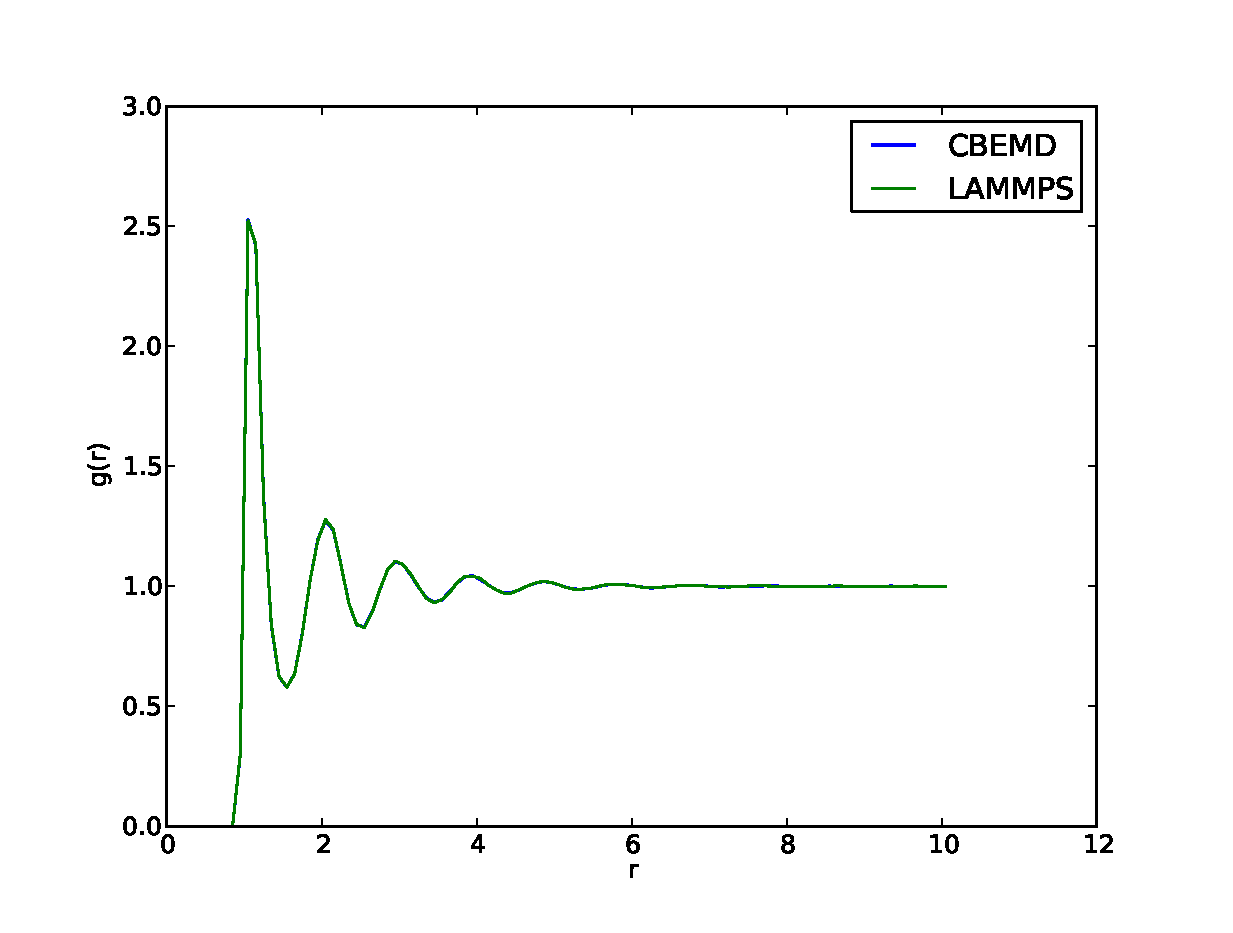
\includegraphics[width=\textwidth]{gr_compare}
	\caption{}
	\end{subfigure}
	\caption{Comparison between CBEMDGPU simulation and LAMMPS simulation for 4000 Lennard Jones particles at $T=0.71$ and $\rho=0.8442$. (a) Comparison of temperature over time. (b) Comparison of potential energy/atom over time. (c) Comparison of total energy/atom over time. (d) Comparison of radial distribution functions. }
	\label{fig:lmp_compare}
\end{figure}

There is excellent agreement between our software (CBEMDGPU) and the LAMMPS results. The average temperature and the behavior of the temperature fluctuations were qualitatively and quantitatively in agreement. Our temperature fluctuations are more smooth since we don't have as much damping and since LAMMPS uses Nos\'{e}-Hoover chains. The potential and total energies' behaviors are the same, and the radial distribution functions calculated in both programs are within numerical error. These results strongly suggest that the software we have developed can largely reproduce the thermodynamic and simulation behavior of the LAMMPS software, and is a strong validation of our underlying code.

\subsection{Example Movie}
To see an example movie of a short LJ fluid simulation, see the file \url{/report/movie1.mpg}.
\section{Conclusions and Future Work}

\pagebreak
\bibliographystyle{proteins1}
\bibliography{references}

\end{document}
